%TODO: Die Schätzungen gehen nur von Veränderungen der verwendeten Menge bzgl.
%Transistoren aus. Wenn diese Menge nur ein Bruchteil ausmacht, dann hat auch
%die Verwendung einer Alternative kaum einen Einfluss. Das müssen wir noch
%irgendwie berücksichtigen.

\section{Wirtschaftlich}\label{sec:conflict}

Dieser Abschnitt beschreibt die wirtschaftliche Nachhaltigkeit von Tantal für alle abgehandelten Szenarien.
\paragraph{Preis}
Mittels Indikator ``Preis'' untersucht man, wie sich der Preis pro Kilo Tantal
in amerikanischen Dollars (USD) verändert. Eine Senkung wird als positiv bewertet, da die ICT-Branche von günstigeren Rohstoffpreisen profitiert. Die Bewertung 5 entspricht dem Tantal-Wert von 2013 (237 USD).

\paragraph{Arbeitsplätze}
Der Indikator ``Arbeitsplätze'' misst, wie die Produktion von Tantal die Anzahl
Arbeitsplätze beeinflusst.

\paragraph{Innovation}
Dieser Indikator misst, ob durch die Produktion von Tental neue Technologien
entstehen und ob diese nachhaltig die Marktentwicklung beeinflussen können.

\paragraph{2013}
Der \textbf{Preis} von Tantal pro Kilogramm betrug im Jahr 2006 65 USD (US Dollars), 2010 121 USD und 2013 237 USD ~\cite{tantal_price2}. 237 USD wird auf der Nachhaltigkeitsskala mit einer 5 eingestuft. 
\\
\begin{figure}[htp]
\centering
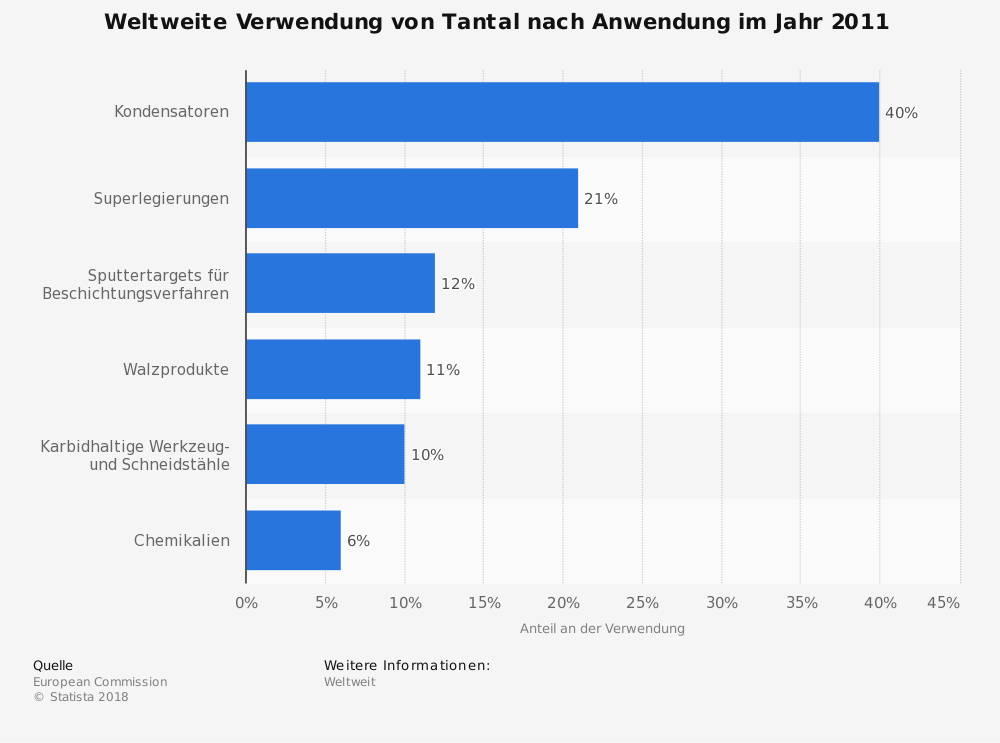
\includegraphics[scale=2.0]{images/tantal_usage_2011.png}
\caption{BGR. n.d. Weltweite Verwendung von Tantal nach Anwendung im Jahr 2011 ~\cite{tantal_usage}}
\label{}
\end{figure}

2013 wurden weltweit 1300 Tonnen Tantal in Bergwerken gefördert ~\cite{tantal_price2}. 2011 wurden 40\% des geförderteten Tantals für Kondensatoren verwendet. Bei gleichbleibender Verwendungsrate entspricht dies einer Fördermenge von 520 Tonnen im Jahr 2013.
% Hier Anzahl Jobs in Verhältnis zu Tonnen bringen. Dann kann man hochrechnen.
\\


\paragraph{2035 bei anhaltendem Trend}
Fliesstext. Indikatoren im Lauftext hervorheben.

\paragraph{2035 mit Kondensatorenalternative}
Fliesstext. Indikatoren im Lauftext hervorheben.

